%%%%%%%%%%%%%%%%%%%%%%%%%%%%%%%%%%%%%%%%%%%%%%%%%%%%%%%%%%%%%%%%%%%%%%
% LaTeX Template: Beamer arrows
%
% Source: http://www.texample.net/
% Feel free to distribute this template, but please keep the
% referal to TeXample.net.
% Date: Nov 2006
% 
%%%%%%%%%%%%%%%%%%%%%%%%%%%%%%%%%%%%%%%%%%%%%%%%%%%%%%%%%%%%%%%%%%%%%%
% How to use writeLaTeX: 
%
% You edit the source code here on the left, and the preview on the
% right shows you the result within a few seconds.
%
% Bookmark this page and share the URL with your co-authors. They can
% edit at the same time!
%
% You can upload figures, bibliographies, custom classes and
% styles using the files menu.
%
% If you're new to LaTeX, the wikibook is a great place to start:
% http://en.wikibooks.org/wiki/LaTeX
%
%%%%%%%%%%%%%%%%%%%%%%%%%%%%%%%%%%%%%%%%%%%%%%%%%%%%%%%%%%%%%%%%%%%%%%

\documentclass{beamer} %
\usetheme{CambridgeUS}
\usepackage[latin1]{inputenc}
\usefonttheme{professionalfonts}
\usepackage{times}
\usepackage{tikz}
\usepackage{amsmath}
\usepackage{verbatim}
\usepackage{multirow}
\usepackage{color}
\newcommand{\blue}[1]{\textcolor{blue}{#1}}
\newcommand{\red}[1]{\textcolor{red}{#1}}
\newcommand{\green}[1]{\textcolor{green}{#1}}
\newcommand{\yellow}[1]{\textcolor{yellow}{#1}}
\newcommand{\orange}[1]{\textcolor{orange}{#1}}




\usetikzlibrary{arrows,shapes}

\author{Nan Meng}
\title{Privacy Preserving Distributed Decision Tree}
\institute[] % Your institution as it will appear on the bottom of every slide, may be shorthand to save space
{
University of Hong Kong \\ % Your institution for the title page
\medskip
\textit{u3003637@connect.hku.hk} % Your email address
}
\begin{document}


% For every picture that defines or uses external nodes, you'll have to
% apply the 'remember picture' style. To avoid some typing, we'll apply
% the style to all pictures.
\tikzstyle{every picture}+=[remember picture]

% By default all math in TikZ nodes are set in inline mode. Change this to
% displaystyle so that we don't get small fractions.
\everymath{\displaystyle}


\begin{frame}
  \titlepage
\end{frame}



% ----------------------------------------------------------------
% ----------------------------------------------------------------
\begin{frame}
\frametitle{Content}
\begin{itemize} \itemsep16pt \parskip0pt \parsep0pt
\item Motivation
\item Distributed Data Mining
\item Privacy Preserving Data Mining
\item Decision Tree
\item Related Works
\item Problem Definition
\end{itemize}
\end{frame}

% ----------------------------------------------------------------

\begin{frame}
\frametitle{Motivation}
\begin{itemize} \itemsep16pt \parskip0pt \parsep0pt
\item Use of \red{\bf technology for data collection} has seen an unprecedented \red{\bf growth} in the last couple of decades. Individuals and organizations generate huge amount of data through everyday activities.
\item \red{\bf Decreasing storage and computation costs} have enabled us to collect data on different aspects of people's lives such as their \blue{\bf credit card transaction records}, \blue{\bf phone call} and \blue{\bf email lists}, \blue{\bf personal health information} and \blue{\bf web browsing habits}
\end{itemize}


\begin{block}{Objective}
{\bf The main objective} in privacy preserving data mining is
to develop algorithms for modifying the original data
in some way, so that the private data and private
knowledge remain private even after the mining process.
\end{block}
\end{frame}
% ----------------------------------------------------------------
% ----------------------------------------------------------------

\begin{frame}
\frametitle{Distributed Data Mining}
\begin{itemize} \itemsep2pt \parskip0pt \parsep0pt
    \item Distributed data mining deals with the problem of data analysis in environments with \red{\bf distributed} data, computing nodes, and users.
    \item Distributed data mining is a field of research that concentrates on \red{\bf developing efficient algorithms} for mining of information from distributed data without centralizing it.
    \begin{itemize} \itemsep2pt \parskip0pt \parsep0pt
        \item[$\ast$] {\bf Algorithms for homogeneous data distribution:} \newline Also known as the {\bf horizontally partitioned scenario}, all attributes or features are observed at every site. However, the set of observations or tuples across the different sites differ.
        \item[$\ast$] {\bf Algorithms for heterogeneous data distribution:} \newline Also known as the {\bf vertically partitioned scenario}, each site has all tuples or rows, but only for a subset of the attributes for the overall data set.
    \end{itemize}
\end{itemize}



\end{frame}
% ----------------------------------------------------------------
% ----------------------------------------------------------------

\begin{frame}
\frametitle{Distributed Data Mining(Intuitive View)}

\begin{itemize} \itemsep2pt \parskip0pt \parsep0pt
    \item[(b)] \red{\bf horizontally} partitioned scenario(homogeneous)
    \item[(c)] \red{\bf vertically} partitioned scenario(heterogeneous)
\end{itemize}


\begin{columns}
\begin{column}{3cm}
\begin{figure}[H]
\centering
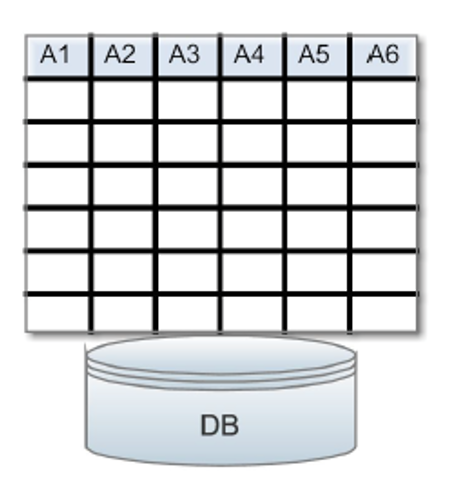
\includegraphics[width=1\textwidth]{./DDM1.png}
\end{figure}
\vspace{2mm}
\centerline{\blue{(a)}}
\end{column}


\begin{column}{5cm}
\begin{figure}[H]
\centering
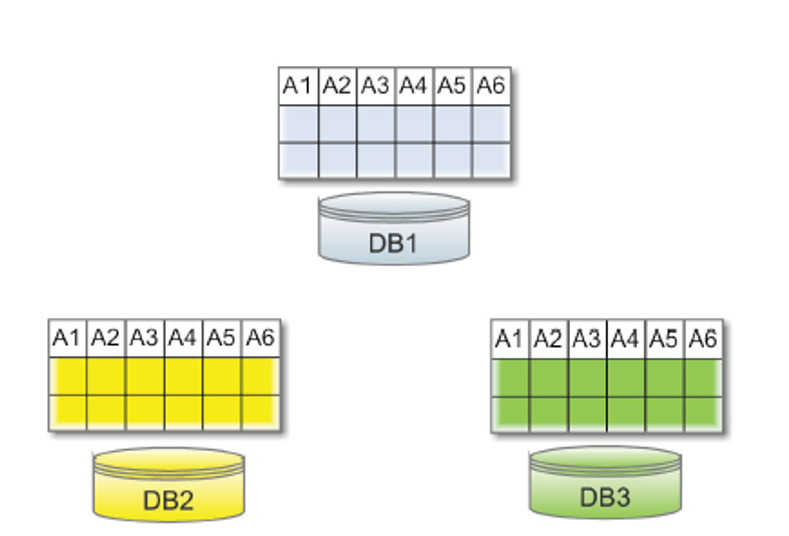
\includegraphics[width=1\textwidth]{./DDM2.png}
\end{figure}
\centerline{\blue{(b)}}
\end{column}


\begin{column}{4cm}
\begin{figure}[H]
\centering
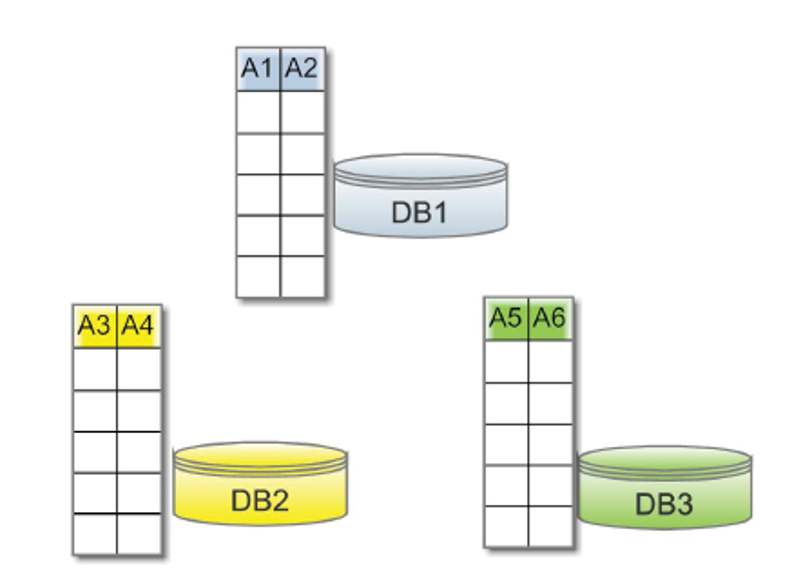
\includegraphics[width=1\textwidth]{./DDM3.png}
\end{figure}
\vspace{4mm}
\centerline{\blue{(c)}}
\end{column}

\end{columns}


\end{frame}
% ----------------------------------------------------------------
% ----------------------------------------------------------------

\begin{frame}
\frametitle{Privacy Preserving Data Mining}
\begin{itemize} \itemsep2pt \parskip0pt \parsep0pt
    \item Privacy preserving data mining, is a novel research  direction  in  data  mining  and  statistical databases, where data mining algorithms are \orange{\bf analyzed for the side-effects} they incur in data privacy.

    \item privacy preserving data mining algorithms can be classified into three categories:
    \begin{itemize} \itemsep2pt \parskip0pt \parsep0pt
        \item {\bf Data distortion based privacy:} Aim at \orange{\bf distorting} the \blue{\bf original private data}, when released, do not divulge any individually identifiable information.
        \item {\bf Cryptography based privacy:} Cryptographic protocols are called private when their execution does \orange{\bf not reveal any additional information} about the involved parties' data, other than what is computed as a result of the protocol execution.
        \item {\bf Output perturbation based privacy:} Output perturbation techniques discuss privacy with respect to the \orange{\bf information released as a result of querying} a statistical database by some external entity.
    \end{itemize}
\end{itemize}



\end{frame}
% ----------------------------------------------------------------
% ----------------------------------------------------------------

\begin{frame}
\frametitle{Privacy Preserving Data Mining(Intuitive View)}

\begin{itemize} \itemsep2pt \parskip0pt \parsep0pt
    \item[$\ast$] Safeguard sensitive information
    \item[$\ast$] Preserve data utility
\end{itemize}
\begin{figure}[H]
\centering
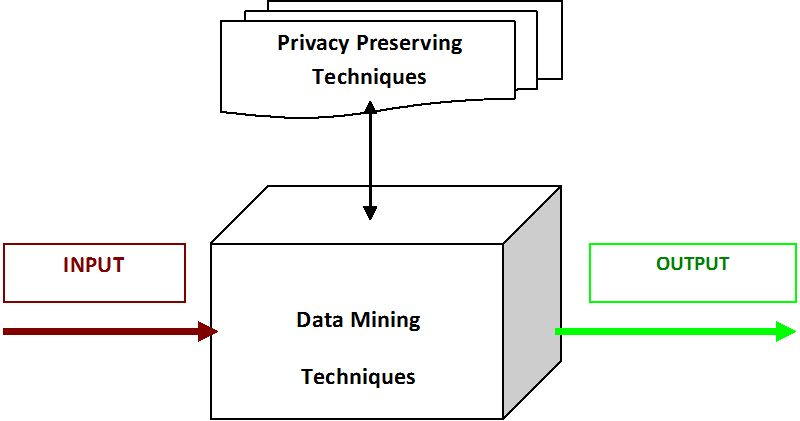
\includegraphics[width=0.8\textwidth]{./PPDM.jpg}
\end{figure}



\end{frame}
% ----------------------------------------------------------------
% ----------------------------------------------------------------

\begin{frame}
\frametitle{Decision Tree(ID3)}
\begin{itemize} \itemsep2pt \parskip0pt \parsep0pt
    \item[] ID3(Iterative Dichotomiser 3) is an algorithm invented by Ross Quinlan used to generate a decision tree from a dataset. The kernel idea of ID3 is to classify samples according to the measurement of ``information entropy'' calculated by greedy algorithm.\newline\newline\newline
    \blue{\bf ID3 Algorithm Steps}
    \begin{itemize} \itemsep1pt \parskip0pt \parsep0pt
        \item[$1$] Calculate the \orange{\bf entropy} of \red{\bf every attribute} using the data set $S$.
        \item[$2$] Split the set $S$ into subsets using the attribute for which \orange{\bf entropy is minimum} (or, equivalently, information gain is maximum).
        \item[$3$] Make a decision tree node containing that attribute
        \item[$4$] Recurse on subsets using remaining attributes.
    \end{itemize}
\end{itemize}



\end{frame}
% ----------------------------------------------------------------
% ----------------------------------------------------------------

\begin{frame}
\frametitle{Related Works}
\begin{itemize} \itemsep2pt \parskip0pt \parsep0pt
    \item[] Secure Multi-party Computation(SMC)
    \item[$1$] Distributed Association Rules Mining Based on SMC
    \begin{itemize} \itemsep2pt \parskip0pt \parsep0pt
        \item[$\ast$] KANTARCIOGLU M,CLIFFTON C.  \orange{{\bf IEEE Trans on Knowledge and Data Engineering, 2004}}\newline ~\blue{Privacy preserving distributed mining of {\bf association rules} on {\bf horizontally partitioned} data}
        \vspace{6mm}
        \item[$\ast$] VAIDYA J, CLIFTON C.  \orange{{\bf ACM SIGMOD 2002}}\newline ~\blue{Privacy preserving {\bf association rules mining} in {\bf vertically partitioned} data}
    \end{itemize}
    \item[$2$] Distributed Clustering Mining Based on SMC

    \item[$3$] Distributed Classification Mining Based on SMC
\end{itemize}



\end{frame}
% ----------------------------------------------------------------
\begin{frame}
\frametitle{Related Works}
\begin{itemize} \itemsep2pt \parskip0pt \parsep0pt
    \item[] Secure Multi-party Computation(SMC)
    \item[$1$] Distributed Association Rules Mining Based on SMC
    \item[$2$] Distributed Clustering Mining Based on SMC
    \begin{itemize} \itemsep2pt \parskip0pt \parsep0pt
        \item[$\ast$] \red{\bf Han Jiawei et al.} proposed two distributed models based on SMC \blue{\bf (Naive model \& Muilt-clustering model)}
        \vspace{6mm}
        \item[$\ast$] \red{\bf JAGANNATHAN G, WRIGHT R N.} proposed \orange{\bf secure-sum} and \orange{\bf secure-means} technique based on SMC
    \end{itemize}
    \item[$3$] Distributed Classification Mining Based on SMC
\end{itemize}

\end{frame}

% ----------------------------------------------------------------
% ----------------------------------------------------------------

\begin{frame}
\frametitle{Related Works}
\begin{itemize} \itemsep2pt \parskip0pt \parsep0pt
    \item[] Secure Multi-party Computation(SMC)
    \item[$1$] Distributed Association Rules Mining Based on SMC
    \item[$2$] Distributed Clustering Mining Based on SMC
    \item[$3$] \red{Distributed Classification Mining Based on SMC}
    \begin{itemize} \itemsep2pt \parskip0pt \parsep0pt
        \item[$\ast$] \red{\bf DU Wen-liang, ZHANG Zhi-jun} proposed the \orange{\bf Privacy Preserving ID3} algorithm(based on SMC) focus on \blue{\bf vertically partitioned data}.
        \vspace{6mm}
        \item[$\ast$] \red{\bf XIAO Ming-jun et al.} proposed the \orange{\bf Privacy Preserving C4.5} algorithm(based on SMC) focus on \blue{\bf horizontally partitioned data}.
    \end{itemize}
\end{itemize}

\end{frame}


% ----------------------------------------------------------------
% ----------------------------------------------------------------


\begin{frame}
\frametitle{Problem Definition}
Consider a {\bf distributed computing environment} consisting of nodes(parties) and connected via an underlying communication infrastructure. 
\begin{itemize} \itemsep2pt \parskip0pt \parsep0pt
    \item[$\ast$] Each node has some data which is known only to itself.
    \item[$\ast$] The nodes can exchange messages with any other node in the network.
\end{itemize}

\vspace{6mm}
This project aims at answering the following question: 
\begin{itemize} \itemsep2pt \parskip0pt \parsep0pt
    \item[$Q:$] how can data mining tasks for \blue{extracting and utilizing useful knowledge} from the \blue{union} of all the data be executed in the system such that different nodes participating in the collaborative computation.
\end{itemize}


\end{frame}

% ----------------------------------------------------------------
% ----------------------------------------------------------------


\begin{frame}
More specifically ...
\begin{itemize} \itemsep2pt \parskip0pt \parsep0pt
    \item[$Q1:$] Can ensure that the required privacy is actually achieved when mining the knowledge of data?
    \item[$Q2:$] Can compute the privacy preserving data mining results with an efficient use of resources?
    \item[$Q2:$] Can realize the system and test it using algorithms?
\end{itemize}
\end{frame}



% ----------------------------------------------------------------
% ----------------------------------------------------------------




\begin{frame}
\Huge{\centerline{\red{Q \& A}}}
\begin{figure}[H]
\centering
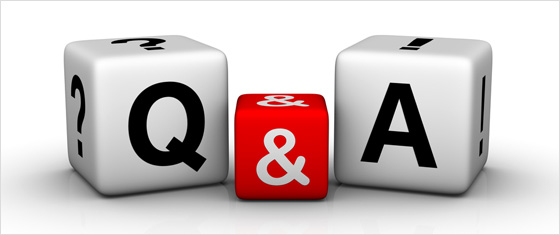
\includegraphics[width=1\textwidth]{./QA.jpg}
\end{figure}
\end{frame}

% ----------------------------------------------------------------
% ----------------------------------------------------------------


\begin{frame}
\Huge{\centerline{The End}}
\end{frame}
\end{document}